\documentclass[12pt,a4paper]{report}
\usepackage[utf8x]{inputenc}
\usepackage{ucs}
\usepackage{amsmath}
\usepackage{amsfonts}
\usepackage{amssymb}
\usepackage{graphicx}
\author{David Navarro Estruch}
\title{Operations Research and Optimization \\ Coursework}

\begin{document}
\maketitle
\chapter{Refinery Optimization}
This problem deals with the optimal way of managing a refinery. The refinery can buy two different crudes. Then it can apply several processes called distillation, reforming, cracking and blending. Each of them needs and produces a variety of subproducts that can be used in another processes.

In the end, our goal is to produce the final products that can be sold at market price. These products are premium petrol, regular petrol, jet fuel, fuel oil and lube oil.

Moreover, the refinery needs to meet several restrictions in the amount of production of some of the products, in the products that can process and in the  crude that can be bought.

Our goal is to use a Linear Programming model to solve and optimize this problem. For this we start describing the algebraic model and the we describe how this model relates to the spreadsheet implemented and with the LP file for the LP solver given.

\section{The algebraic model}
To start we are going to describe all the variables that we are going to use. Then we will continue enumerating the different constraints and boundaries.
\subsection{Variables}
We use abbreviations for all the variables. These abbreviations are used to keep the mathematical formulas short and concise. They are also used in the spreadsheet model but there are annotations in all of them to help the users.

All the variables are real positive numbers.

Here is a list of all the variables with their meaning. Their use is explained in the constraints.

First the abbreviations of the crude that can be bought
\begin{description}
\item[CRA]
Crude 1
\item[CRB]
Crude 2
\end{description}

Next the abbreviations of the final products
\begin{description}
\item[PMF]
Premium motor fuel
\item[RMF]
Regular motor fuel
\item[JF]
Jet fuel
\item[FO]
Fuel oil
\item[LBO]
Lube-oil
\end{description}

Finally we introduce the abbreviation of the intermediate variables. These comprises both the derived subproducts that cannot be sold and some extra variables needed to implement the Linear Programming model.
\begin{description}
\item[LN]
Light naphtha 
\item[MN]
Medium naphtha 
\item[HN]
Heavy naphtha 
\item[LO]
Light oil
\item[HO]
Heavy oil
\item[R]
Residuum
\item[LNRG]
Light naphtha used to produce reformed gasoline
\item[MNRG]
Medium naphtha used to produce reformed gasoline
\item[HNRG]
Heavy naphtha used to produce reformed gasoline
\item[RG]
Reformed gasoline
\item[LOCGO]
Light oil used to produce cracked oil and cracked gasoline
\item[HOCGO]
Heavy oil used to produce cracked oil and cracked gasoline
\item[CG]
Cracked gasoline
\item[CO]
Cracked oil
\item[LNPMF]
Light naphtha used to produce premium motor fuel
\item[LNRMF]
Light naphtha used to produce regular motor fuel
\item[MNPMF]
Medium naphtha used to produce premium motor fuel
\item[MNRMF]
Medium naphtha used to produce regular motor fuel
\item[HNPMF]
Heavy naphtha used to produce premium motor fuel
\item[HNRMF]
Heavy naphtha used to produce regular motor fuel
\item[RGPMF]
Reformed gasoline used to produce premium motor fuel
\item[RGRMF]
Reformed gasoline used to produce regular motor fuel
\item[CGPMF]
Cracked gasoline used to produce premium motor fuel
\item[CGRMF]
Cracked gasoline used to produce regular motor fuel
\item[LOJF]
Light oil used to produce jet fuel
\item[HOJF]
Heavy oil used to produce jet fuel
\item[RJF]
Residuum used to produce jet fuel
\item[COJF]
Cracked oil used to produce jet fuel
\item[RLBO]
Residuum used to produce lube-oil
\end{description}

We are not going to require the variables that decides how much of materials we are going to need to make fuel oil. Fuel oil is made on fixed proportions. The amount of light oil used to make fuel oil can be calculated multiplying the fuel oil for the proportion of light oil. This calculation is linear and legal in our model. With this observation the use of variables for computing this values can be avoided.

\subsection{Boundaries}

We are going to introduce all constraints. The constraints will be explained when further explanation would improve the understanding of the description from the book.

In addition to the non-negativity constraint and the fact that all the variables have to be positive we have the following boundary constraints.

\begin{equation}
CRA\leq 20,000
\end{equation}
\begin{equation}
CRB\leq 30,000
\end{equation}
\begin{equation}
500 \leq LBO \leq 1,000
\end{equation}
\subsection{Constraints}

The next constraints describe amounts that need to be preserved in the different transformation. The books equals of the equations to zero. We are going to move the variables to both sides of the equation reflecting more closely the problem. This approach is the same we used in the spreadsheet. In our humble opinion, this will help the readers who are more familiar with the problem domain than with this approach.

In general, the equations means that some material on the left can be transformed by some process in the materials of the right.
\begin{align}
CO &= 0.68\ LOCGO + 0.75\ HOCGO\\
CG &= 0.28\ LOCGO + 0.2\ HOCGO
\end{align}

\begin{equation}
LBO = 0.5\ RLBO
\end{equation}

In other equations we are assigning some resource to several variables. These equations check that the naphtha is split in all the uses. These do not represent a industrial process.
\begin{align}
LN &= LNRG + LNPMF + LNRMF\\
MN &= MNRG + MNPMF + MNRMF\\
HN &= HNRG + HNPMF + HNRMF
\end{align}

In these equations it is used the concept of the proportion mentioned before. In the first four equations we want to check how the material is split between its uses. There is not a variable for the amount of material used for fuel oil but we can compute the value give the amount produced and the ratio.

The $CG$ and $RG$ equations are the usual split between their respective uses.
\begin{align}
LO &= LOCGO + LOJF + \frac{10}{18}\ FO\\
CO &= COJF + \frac{4}{18}\ FO\\
HO &= HOCGO + HOJF + \frac{3}{18}\ FO\\
R &= RJF + RLBO + \frac{1}{18}\ FO\\
CG &= CGPMF + CGRMF\\
RG &= RGPMF + RGRMF
\end{align}

These equations represent the amount of final materials created given the products used.
\begin{align}
PMF =& LNPMF + MNPMF +\notag\\
     & HNPMF + RGPMF + CGPMF\\
RMF =& LNRMF + MNRMF +\notag\\
     & HNRMF + RGRMF + CGRMF\\ 
JF  =& LOJF + HOJF + RJF + COJF
\end{align}

Finally the next equations reflects the capacities, qualities and other criteria that have to be fulfilled but do not need an equality.
\begin{equation}
CRA + CRB \leq 45,000
\end{equation}
\begin{equation}
LNRG + MNRG + HNRG \leq 10,000
\end{equation}
\begin{equation}
LOCGO + HOCGO \leq 8,000
\end{equation}
\begin{equation}
PMF \geq 0.4\ RMF
\end{equation}
These equations checks that the motor fuel created matches the requirements on the octane number. The last checks that the vapour pressure is low enough in the jet fuel.
\begin{align}
94\ PMF \leq & 90\ LNPMF + 80\ MNPMF + \notag\\
             & 70\ HNPMF + 115\ RGPMF + 105\ CGPMF\\
84\ RMF \leq & 90\ LNRMF + 80\ MNRMF + \notag\\
             & 70\ HNRMF + 115\ RGRMF + 105\ CGRMF\\
JF    \geq &LOJF + 0.6\ HOJF + 1.5\ COJF + 0.05\ RJF
\end{align}
\subsection{Objective function}
In this problem we want to \textit{maximize} the profit. The profit is found
by the amount of each final product produced and its price. This leads to the following
objective function.
\begin{equation}
max:\quad 7\ PMF + 6\ RMF + 4\ JF + 3.5\ FO + 1.5\ LBO
\end{equation}

\section{The spreadsheet}
The organization of the spreadsheet looks to get easy of use even for people who don't understand the modelization. 

There is a legend that explains all the colors that have been used to help people to find what they are looking.

We have also explained every configuration cell and the effect it has. We have tried to keep the number of configuration options low. This way should be easier to change the spreadsheet most of the times.

For the people who do not know the modelization we have placed the most important data on the top left of the spreadsheet so people who start reading there don't need to read anymore.

All the configuration can be found easily by the color.

The most important data is the \textbf{solution found} and the \textbf{crude bought}. This data is found in the first two columns. This corresponds to the data found in the Variables section. Each value has a explanation of what the abbreviation means.

The benefits of each product is configurable in the next column.

At the bottom you can find the profit configuration and the profit found in the given solution. This correspond to the 1.33 formula which is the \textbf{objective function}.

The next column on the right is all the \textbf{intermediate products}. All of them have a
note explaining what the abbreviation means. All of them are the same as defined in the Variables section.

The remaining columns are for the calculation of the restrictions. 

The crude column is devoted to the \textbf{boundaries}. These correspond to the
boundaries with formulas (1.1 - 1.3). This column is also devoted to capacities, availabilities and qualities. These correspond to formulas (1.26, 1.27, 1.28, 1.30, 1.31 1.32).

The last column shows all the \textbf{other restrictions}. The column expresses first the name that
is in the left of the equality, then the formula in the right and at the end the formula in the end. The formulas correspond to 1.4 to 1.25. The formulas are organized in the same
order in the report and in the spreadsheet so they are easy to find.

At the bottom of the last column is the missing restriction, 1.29, corresponding to the
restriction on the amount of premium fuel produced considering the amount of regular fuel.

The characteristics of each kind of crude can be found at the bottom right and correspond to the composition the crudes.

This summarizes all the information of the spreadsheet.

\chapter{Three dimensional Noughts and Crosses}
This problem deals with the best way to arrange black and white balls in a three dimensional cube of 27 squares. The balls can be located on each cube, even if it is in the middle.

The lines are straight lines that comprises parallel lines to the axis, $45$ degrees on one of the axis and $45$ on two of the axis. The parallel lines leads to $9$ lines in each dimension, giving us $9\times 3$ lines. The $45$ degrees gives us $6$ each dimension which leads to $6\times 3$ and the $45$ degrees in two dimensions gives us $4$ extra. This adds up to $49$ lines.

There is an additional restriction that says that 14 black balls and 13 white balls will be used. This also means that all the boxes would be used. We only need to know which color are they going to hold.
\section{The algebraic model}
\subsection{Variables}
For this problem we want to use all the boxes with two states. For this we can use binary variables. We choose that 0 means white ball and 1 means black ball. There are 27 boxes. So we use the next variables:

\begin{equation}
\delta_j = \left\lbrace 0, 1\right\rbrace\quad\quad \forall j \in \left\lbrace 1\dots 27\right\rbrace
\end{equation}

The way of annotating they is better explained in this picture:
\begin{figure}[ht]
\begin{center}
%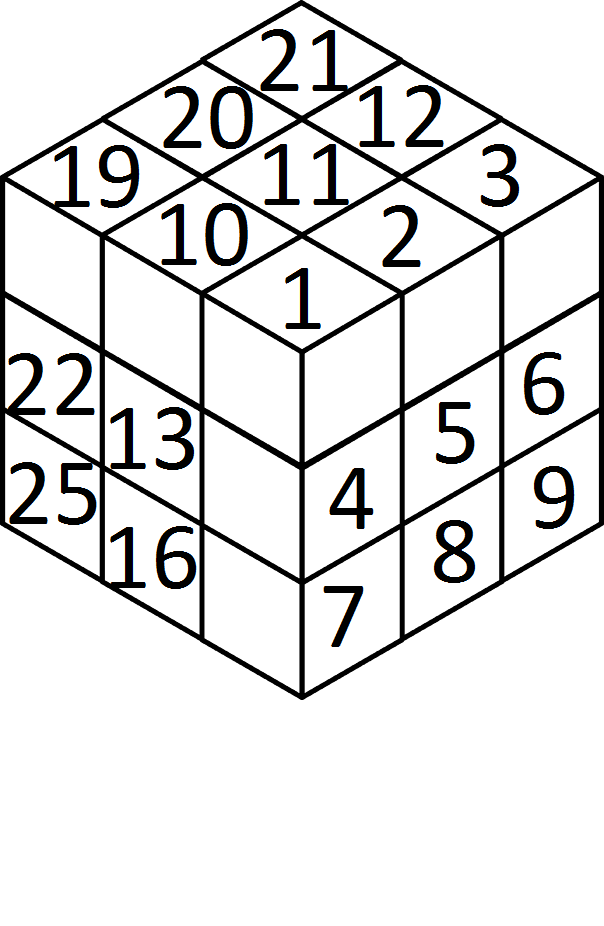
\includegraphics[scale=0.4]{schemaoro.png} 
\end{center}
\caption{Index of the numbering of the boxes in the cube}
\end{figure}

The description of the lines are before. We have numerated them following the order of the description. Each line can be occupied by three balls of the same color or not. This leads again to binary variables. The lines are $49$ so they are numbered

\begin{equation}
\gamma_i = \left\lbrace 0, 1\right\rbrace\quad\quad \forall i \in \left\lbrace 1\dots 49\right\rbrace
\end{equation}

The lines follows the order of the explanation before.

In this problem as all the variables are binary we do not have any boundary constraints in addition to the domain.

\subsection{Constraints}

Using the notation of the book we want that 

$\gamma_i = 0 \Leftrightarrow \delta_{\sigma(i,1)} + \delta_{\sigma(i,2)} + \delta_{\sigma(i,3)} \geq 1 $ or $\delta_{\sigma(i,1)} + \delta_{\sigma(i,2)} + \delta_{\sigma(i,3)} \leq 2$ with $\sigma(i,j)$ being the index of the $j$ box in the $i$ line.

So our constraints are:
\begin{align}
\delta_{\sigma(i,1)} + \delta_{\sigma(i,2)} + \delta_{\sigma(i,3)} - \gamma_i &\leq 2\\
\delta_{\sigma(i,1)} + \delta_{\sigma(i,2)} + \delta_{\sigma(i,3)} + \gamma_i &\geq 1
\end{align}

This equation comprises $49\times 2 = 98$ restrictions.

This avoid the definition of the $\delta$ function. This function can be described by a set of functions depending of the number of the line and multiples of $j$. This definition is not worthy in this problem as the amount of formulas is bigger than just following the lines in the given figure.

The last restriction is in the number of balls of each color. We want only $14$ black balls. As the variables are binary this can be achieved with the following restriction:

\begin{equation}
\sum_{j=1}^{27} \delta_j = 14
\end{equation}

\subsection{Objective function}
In this problem we want to minimize the amount of lines that have all the balls with the same colour. The lines with all lines of the same colour are represented by $\gamma_i = 1$. So our objective function is:

\begin{equation}
min:\quad \sum_{j=1}^{49} \gamma_j
\end{equation}
\section{The spreadsheet}
This problem has less differences between the variables than the first one and the spreadsheet is easy to understand.

The first column correspond to all the cells. The second and third columns correspond to
all the lines.

The next columns correspond to the constraints of the lines. The first two columns
for the line to be 1 when all are white. This checks the constraint 2.4. The next two for the line to be 1 when all are black. And is represented in the model by the constraint 2.3.

At the bottom there is the amount of balls black balls available for configuration. There is also the amount of balls used. These to values are used to represent the 2.5 equation.

The yellow cell computes the objective function. This is the 2.6 equation.

The spreadsheet has some instructions in the right including a figure that helps the user to understand how to interpret the result.
\end{document}
